\section{Расчетно-конструкторская часть}
    \subsection{Расчет основных параметров двигателя}
        Пусковой ток
        \begin{gather*}
            I_\text{п} = 5,5 \cdot I_\text{н},\\
            I_\text{п} = 5,5 \cdot 0,76 = 4,18 \; \text{А}.
        \end{gather*}

        Номинальное скольжение
        \begin{gather*}
            S_\text{н} = \frac{n_0 - n_\text{н}}{n_0},\\
            S_\text{н} = \frac{1500 - 1350}{1500} = 0,1.
        \end{gather*}

        Критическое скольжение
        \begin{gather*}
            S_\text{кр} = S_\text{н} \cdot
                \left( \lambda_{max} + \sqrt{\lambda_{max}^2 - 1} \right),\\
            S_\text{кр} = 0,1 \cdot
                \left( 2,1 + \sqrt{2,1^2 - 1} \right) = 0,416.
        \end{gather*}

        Номинальный момент
        \begin{gather*}
            M_\text{н} = \cfrac{P_\text{н}}
                {2\pi \cdot \cfrac{n_\text{н}}{60}},\\
            M_\text{н} = \frac{120}{2\pi \cdot \cfrac{1350}{60}}
                = 0,849 \; \text{Н} \cdot \text{м}.
        \end{gather*}

        Вычислим максимальный момент двигателя
        \begin{gather*}
            M_{max} = \lambda \cdot M_\text{н},\\
            M_{max} = 2,2 \cdot 0,849 = 1,867 \; \text{Н} \cdot \text{м}.
        \end{gather*}

        Найдем сопротивление статора
        \begin{gather*}
            R_s = \frac{\left(\cfrac{U_\text{н}}{\sqrt{3}}\right)
                \cdot (1 - S_\text{н}) \cdot 1,5}{c_1 \cdot
                    \left(1+\cfrac{c_1}{S_\text{кр}}\right) \cdot
                        M_{max} \cdot (P_\text{н} + \Delta P_\text{Т})},\\
            R_s = \frac{\left(\cfrac{220}{\sqrt{3}}\right) \cdot (1-0,1)
                \cdot 1,5}{1,026 \cdot \left(
                   1+\cfrac{1,026}{S_\text{кр}}\right) 1,867 \cdot
                        (120 + DP_T)} = 0,18 \; \text{Ом}
        \end{gather*}

        Найдем сопротивление ротора
        \begin{gather*}
                R_r = \frac{P_\text{н} + \Delta P_\text{Т}}
                    {3 \cdot (1-S_\text{н}) \cdot i_\text{к}^2
                        \cdot I_\text{н}^2},\\
                R_r = \frac{P_\text{н} + \Delta P_\text{Т}}
                    {3 \cdot (1-S_\text{н}) \cdot i_\text{к}^2
                        \cdot I_\text{н}^2} = 0,15 \; \text{Ом}.
        \end{gather*}

        Расчитаем индуктивность статора
        \begin{gather*}
            L_s = \frac{\cfrac{U_\text{н}}{\sqrt{3} \cdot
                (2\pi \cdot f \cdot I_\text{н})}}{\sqrt{1 - \cos^2 f}
                    - \cos f \left(\cfrac{S_\text{н}}{S_\text{кр}}\right)},\\
            L_s = \frac{\cfrac{220}{\sqrt{3}} \cdot
                (2\pi \cdot 50 \cdot 0,76)}{\sqrt{1 - 0,66^2}
                    - 0,66 (0,416)} = 0,0043 \; \text{Гн}.
        \end{gather*}

        Рассчитаем индуктивность ротора
        \begin{gather*}
            L_r = L_s,\\
            L_r = 0,0043 \; \text{Гн}.
        \end{gather*}

        Индуктивность намагничивания
        \begin{gather*}
            L_m = L_s - L_{1s} = 0,00382 \; \text{Гн}.
        \end{gather*}

        Конструктивная постоянная
        \begin{gather*}
            clr = 1+\frac{L_{1s}}{L_m} = 0,0109.
        \end{gather*}

        Вычислим время разгона
        \begin{gather*}
            t_\text{р} = \frac{\omega_\text{н}}{
                \cfrac{M_\text{н}}{j}} = 0,13 \; \text{с}.
        \end{gather*}

        Вычислим номинальную угловую скорость
        \begin{gather*}
            \omega_\text{н} = \frac{2\pi n_\text{н}}{60} 
                = \frac{2 \cdot 3,14 \cdot 1350}{60} = 141 \; \text{мин}^{-1}.
        \end{gather*}

        Вычислим скорость идеального холостого хода
        \begin{gather*}
            \omega_0 = \frac{2\pi n_0}{60} 
                = \frac{2 \cdot 3,14 \cdot 1500}{60} = 157 \; \text{мин}^{-1}.
        \end{gather*}

        Индуктивное сопротивение статора
        \begin{gather*}
            X_s = 2\pi \cdot 50 \cdot L_s
                = 6,28 \cdot 50 \cdot 0,0043 = 1,35 \text{Ом}.
        \end{gather*}
        
        Индуктивное сопротивление ротора
        \begin{gather*}
            X_r = 2\pi \cdot 50 \cdot L_r
                = 6,28 \cdot 50 \cdot 0,0043 = 1,35 \text{Ом}.
        \end{gather*}
    \subsection{Разработка аппаратной части системы управления автономным
        инвертором напряжения}

%        Разработанная система управления построена на основе отладочного модуля
%        микроконтроллеров серии STM32F100х фирмы ST Microelectronics.

        Блок управления автономным инвертором напряжения реализует
        модулирование ШИМ сигнала управления трехфазным мостом синусоидальным
        сигналом переменной частоты и амплитуды. Амплитуда и частота
        синусоидального сигнала изменяются в соответствии со скалярным законом
        регулирования частоты вращения ротора асинхронного двигателя с
        постоянством отношения $U/f$.

        Принципиальная электрическая схема системы управления АИН представленна
        на рисунке \ref{fig:control-schematic}.

        \begin{sidewaysfigure}
            \center{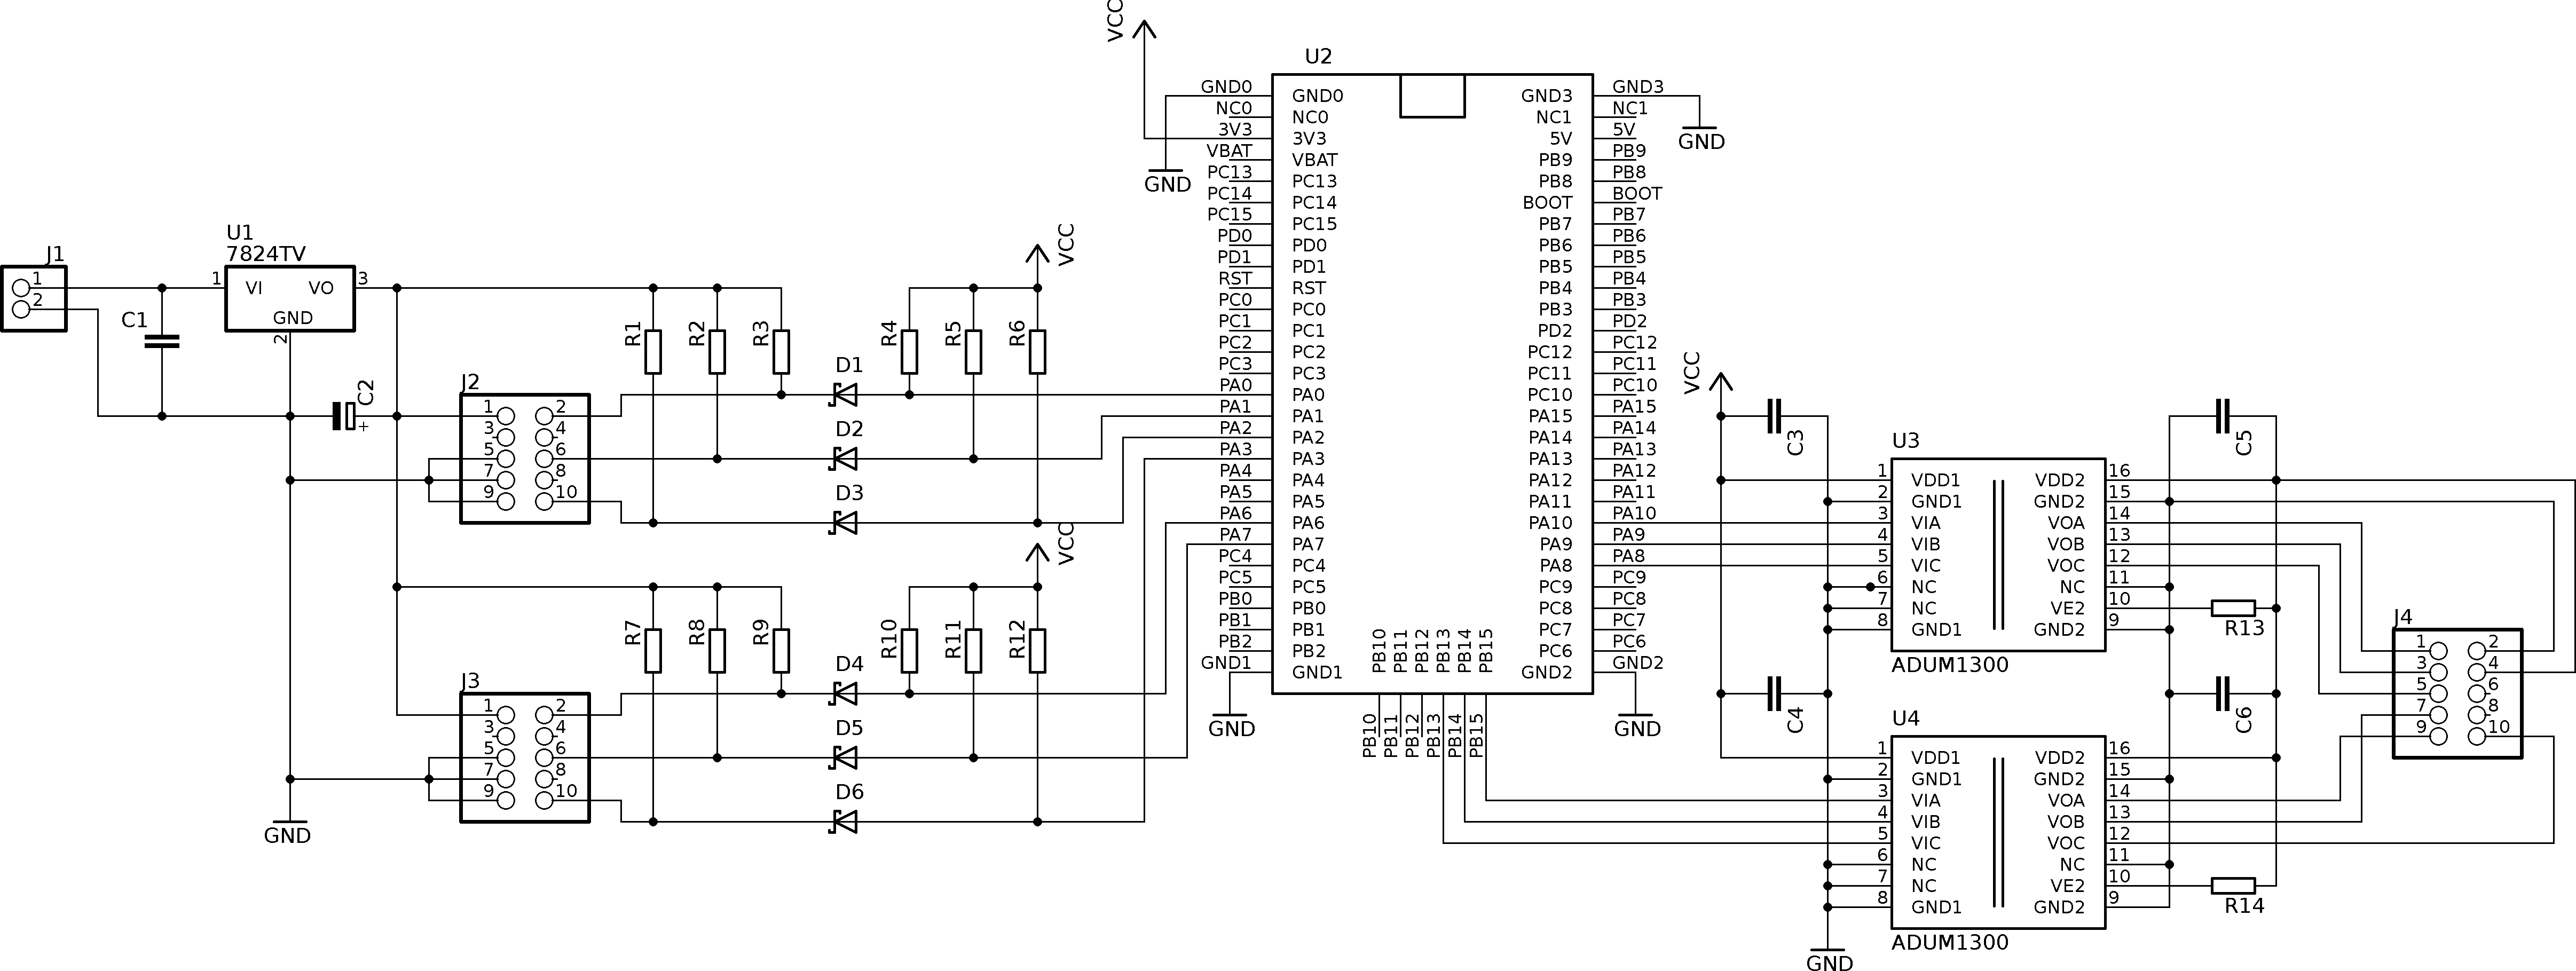
\includegraphics[width=1.0\linewidth]{img/control-schematic}}
            \caption{Принципиальная электрическая схема блока управления АИН}
            \label{fig:control-schematic}
        \end{sidewaysfigure}

        Сигнал управления трехфазным мостом силовых транзисторов АИН снимается
        с выводов PA8, PA9, PA10 (верхние транзизторы моста; фаза A, B и C
        соответственно) и PB13, PB14, PB15 (фаза A, B и C; нижние транзисторы).
        Далее сигнал подается на схему гальванической развязки выполненную на
        двух микросхемах U3 и U4. 
        
        Гальваническая развязка силового блока и блока управления необходима
        так как потенциал общего провода силовой части электропривода может
        иметь значение напряжения питающей сети. Поэтому применением цифровх
        изоляторов с напряжением пробоя болле 2 КВ, обеспечивается защита
        оператора установки от поражения электрическим током, а так же
        буферизация и защита модуля управления от аватийных ситуаций в силовой
        части АИН.

        Конденсаторы С3 - С6 выполняют роль блокировочных, предупреждая броски
        тока в цепяи питания. Резисторы R13 и R14 обеспечивают подтяжку к
        напряжению питания входов разрешения работы цифровых изоляторов.

        Блок управления получает сигналы с двух датчиков скрости через схему
        согласования уровней, выполненную на элементах R1 - R12 и D1 - D6.
        Напряжение питания датчиков скорости снимается с линейного
        интегрального стабилизатора LM7824.

        Конструктивно блок управления выполнен на печатной плате из
        стеклотекстолита толщиной 1,5 мм. Чертеж печатной платы приведен на
        рисунке \ref{fig:control-board-route}. Расоложение элементов -- на
        рисунке \ref{fig:control-board-place}.

        \begin{figure}[h!]
            \center{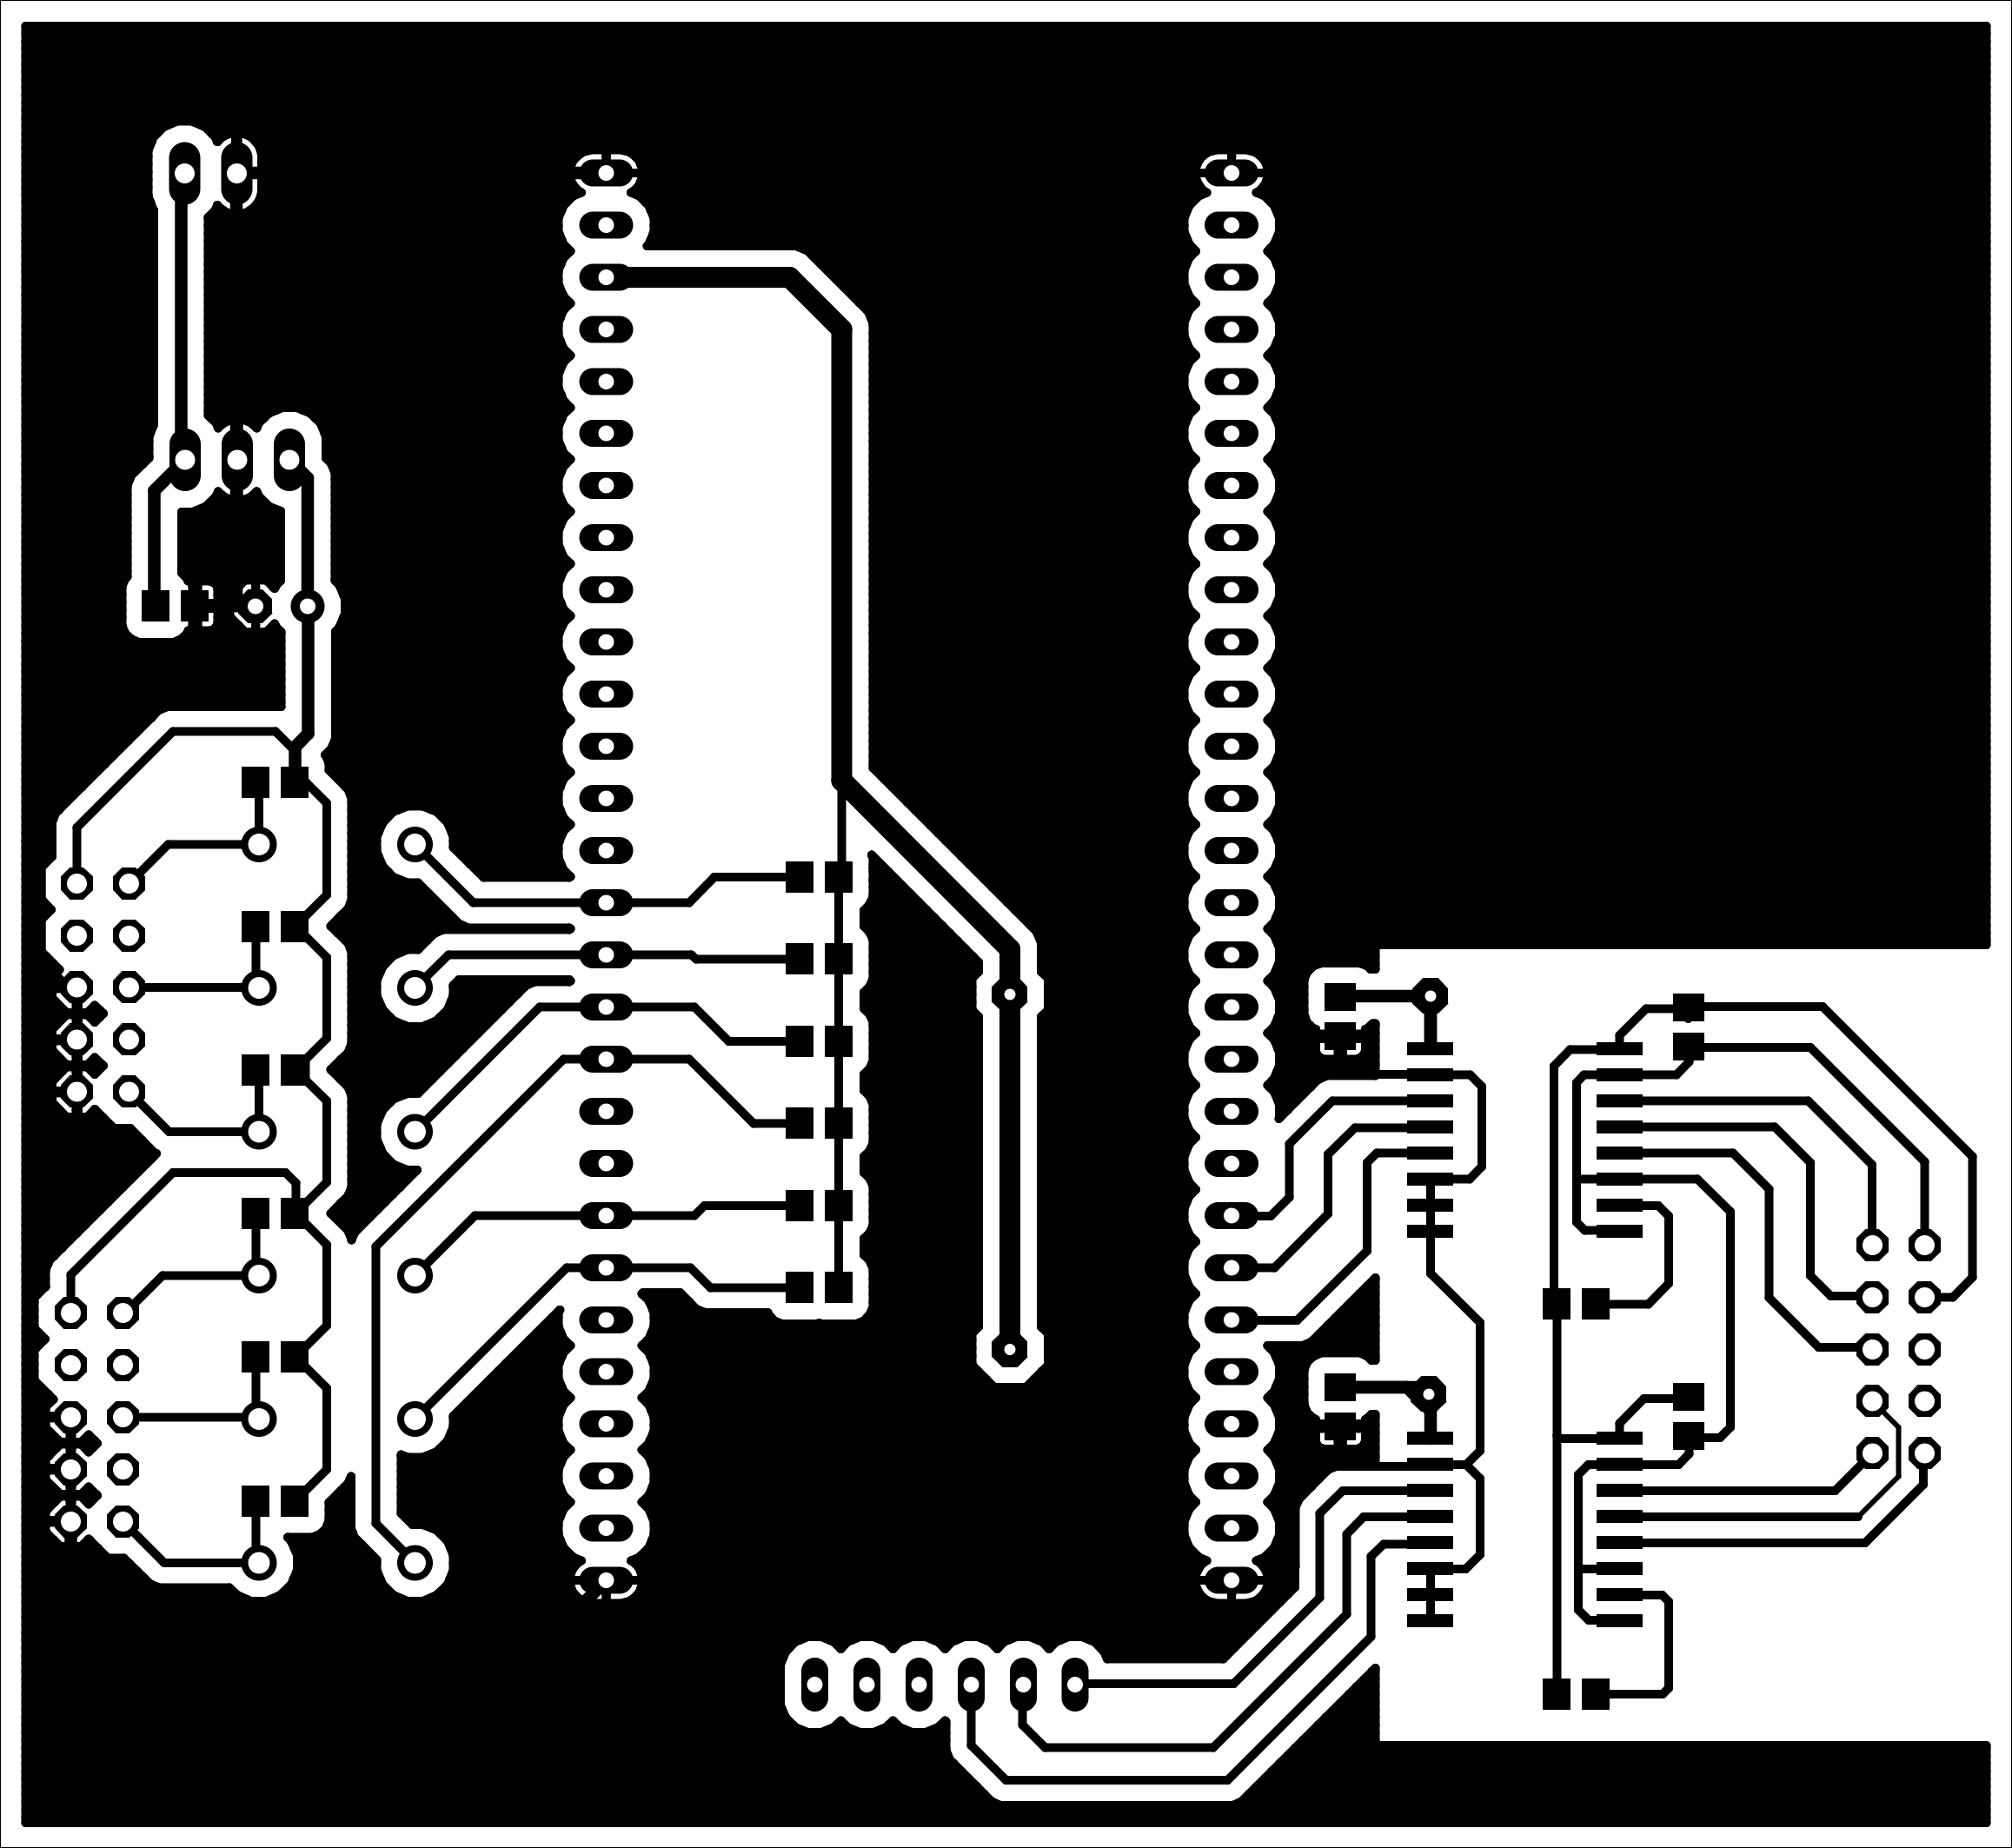
\includegraphics[width=0.8\linewidth]{img/control-board-route}}
            \caption{Чертеж печатной платы блока управления АИН}
            \label{fig:control-board-route}
        \end{figure}

        \begin{figure}[h!]
            \center{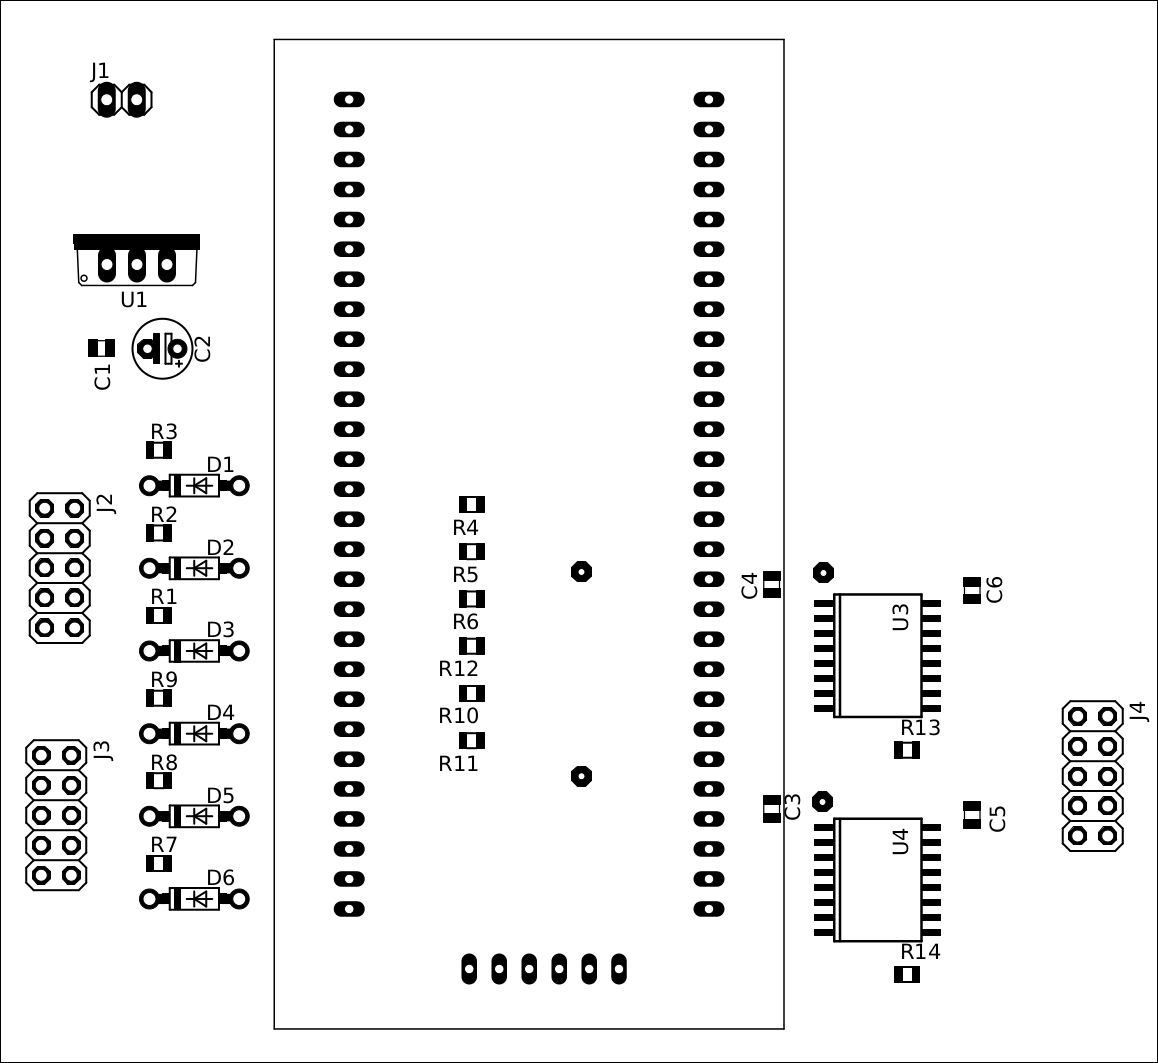
\includegraphics[width=0.8\linewidth]{img/control-board-place}}
            \caption{Схема расположения элементов блока управления АИН}
            \label{fig:control-board-place}
        \end{figure}
        
    \subsubsection{Описание модуля STM32VLDiscovery}
        STM32VLDiscovery -- встраиваемый модуль с интегрированным\\
        JTAG-отладчиком на базе микроконтроллера STM32F100RBT6B семейства STM32
        Value Line. Работа с платой поддерживается в интегрированной среде
        разработки компаний IAR, Keil, Atollic, а также свободным набором
        компиляторов GNU Compiler Collection.

        Установленный микроконтроллер в 64-выводном корпусе LQFP работает на
        частоте 24 МГц. Плата имеет разъем расширения, который позволяет
        подключать ее к другим отладочным платформам для более глубокого
        анализа работы периферии микроконтроллера или к макетным платам для
        прототипирования.

        Установленный на плате отладчик/программатор ST-Link, может
        использоваться как для внутрисхемного программирования встроенного
        микроконтроллера так и в качестве отдельного устройства.

        Отличительные особенности:
        \begin{itemize}
            \item на плате имеется внутрисхемный отладчик/программатор ST-Link;
            \item USB интерфейс ко встроенному отладчику;
            \item переключатель для использования платы в качестве отдельного
                устройства ST-Link;
            \item питание возможно от USB интерфейса или от внешнего источника; 
            \item два светодиода индикации состояния;
            \item два пользовательских светодиода, пользовательская кнопка,
                кнопка \\ <<Сброс>>;
            \item коннектор расширения – доступны все линии ввода/вывода
                микроконтроллера, может использоваться для подключения к
                макетной плате или другой отладочной системе.
        \end{itemize}

        Внешний вид, расположение элементов и размеры модуля приведены на
        рисунке \ref{fig:stm32vldiscovery}.

        \begin{sidewaysfigure}
            \center{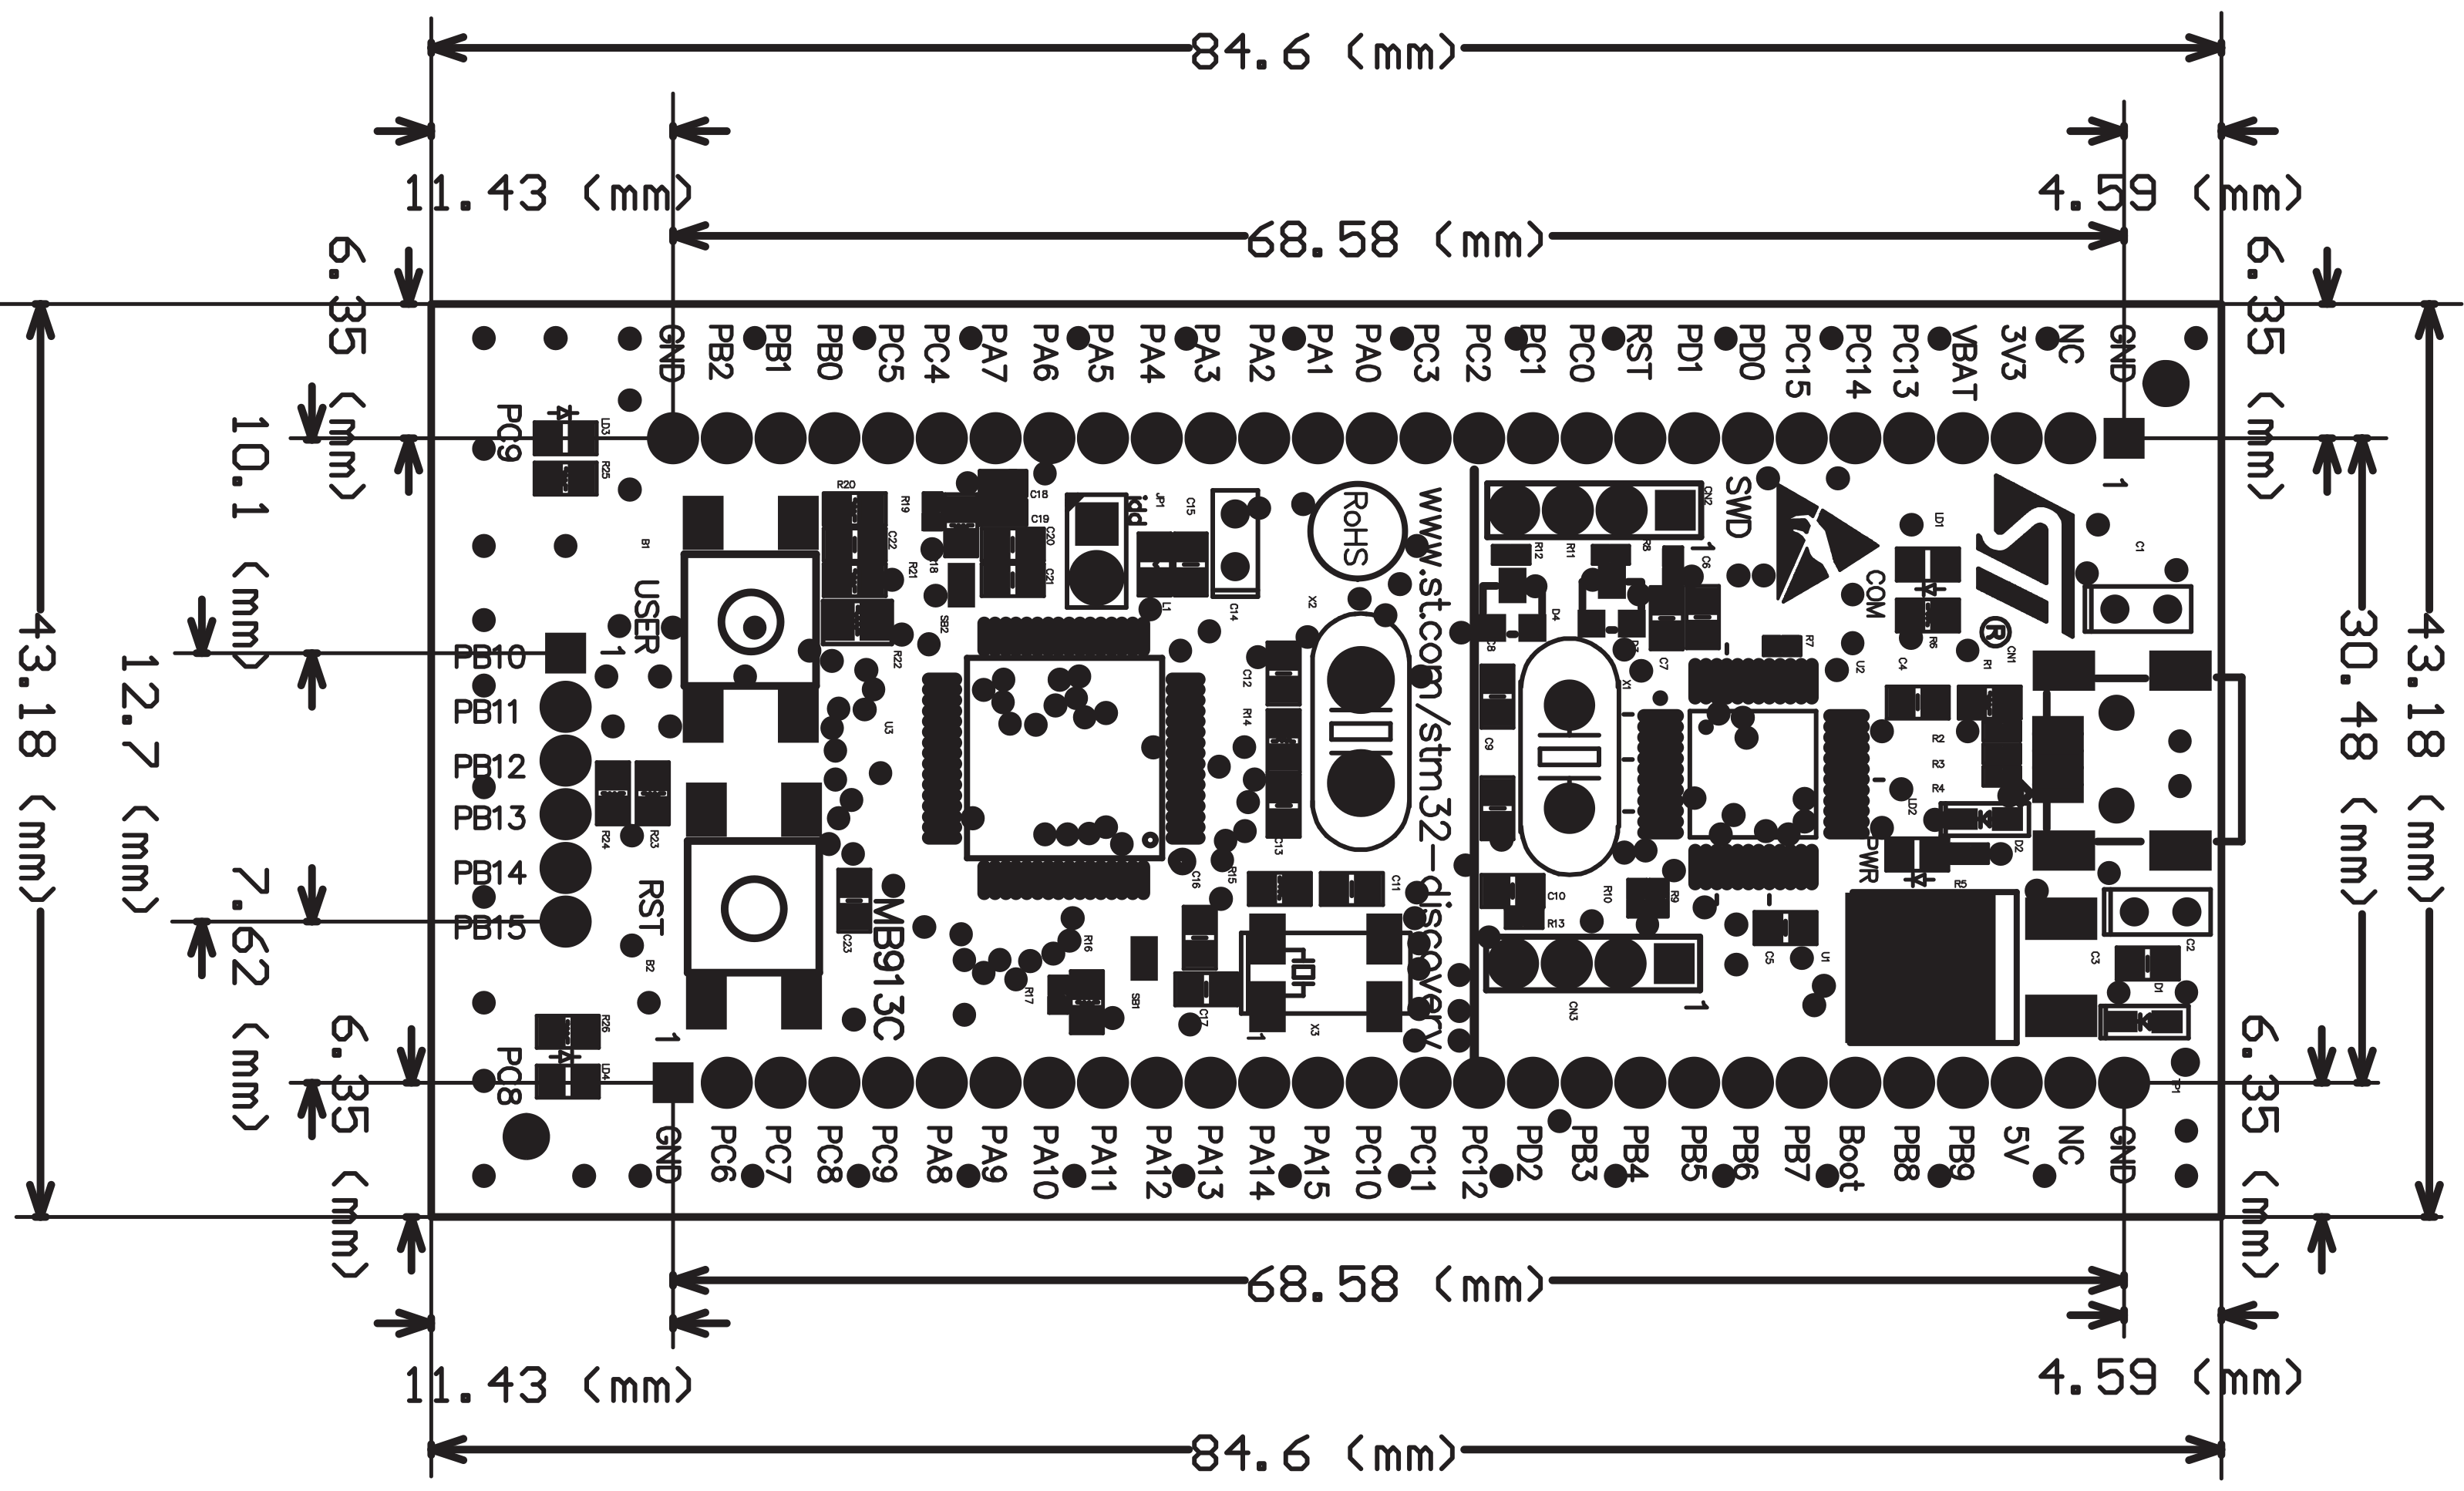
\includegraphics[width=0.8\linewidth]{img/stm32vldiscovery}}
            \caption{Размеры и расположение элементов модуля STM32VLDiscovery}
            \label{fig:stm32vldiscovery}
        \end{sidewaysfigure}       

    \subsubsection{Описание микроконтроллера STM32F100RBT6B}
        Особенности микроконтроллера STM32F100R:
        \begin{itemize}
            \item Вычислительное ядро Cortex-M3;
            \item Максимальная тактовая частота: 24 МГц;
            \item Напряжение питания 2,0 — 3,6 В;
            \item 128 кбайт NOR flash памяти с количеством циклов перезаписи 10000;
            \item 8 кбайт статической оперативной памяти;
            \item 7-канальный контроллер прямого доступа в память;
            \item 51 линия портов ввода-вывода общего назначения;
            \item 12-битный 16-канальный АЦП с временем преобразования 1,2 мкс;
            \item 12-битный ЦАП;
            \item 16-битный таймер с расширенными функциями;
            \item шесть 16-битных таймеров общего назначения;
            \item Восемь коммуникационных интерфейсов (I2C, USART, SPI).
        \end{itemize}

        \begin{sidewaysfigure}
            \center{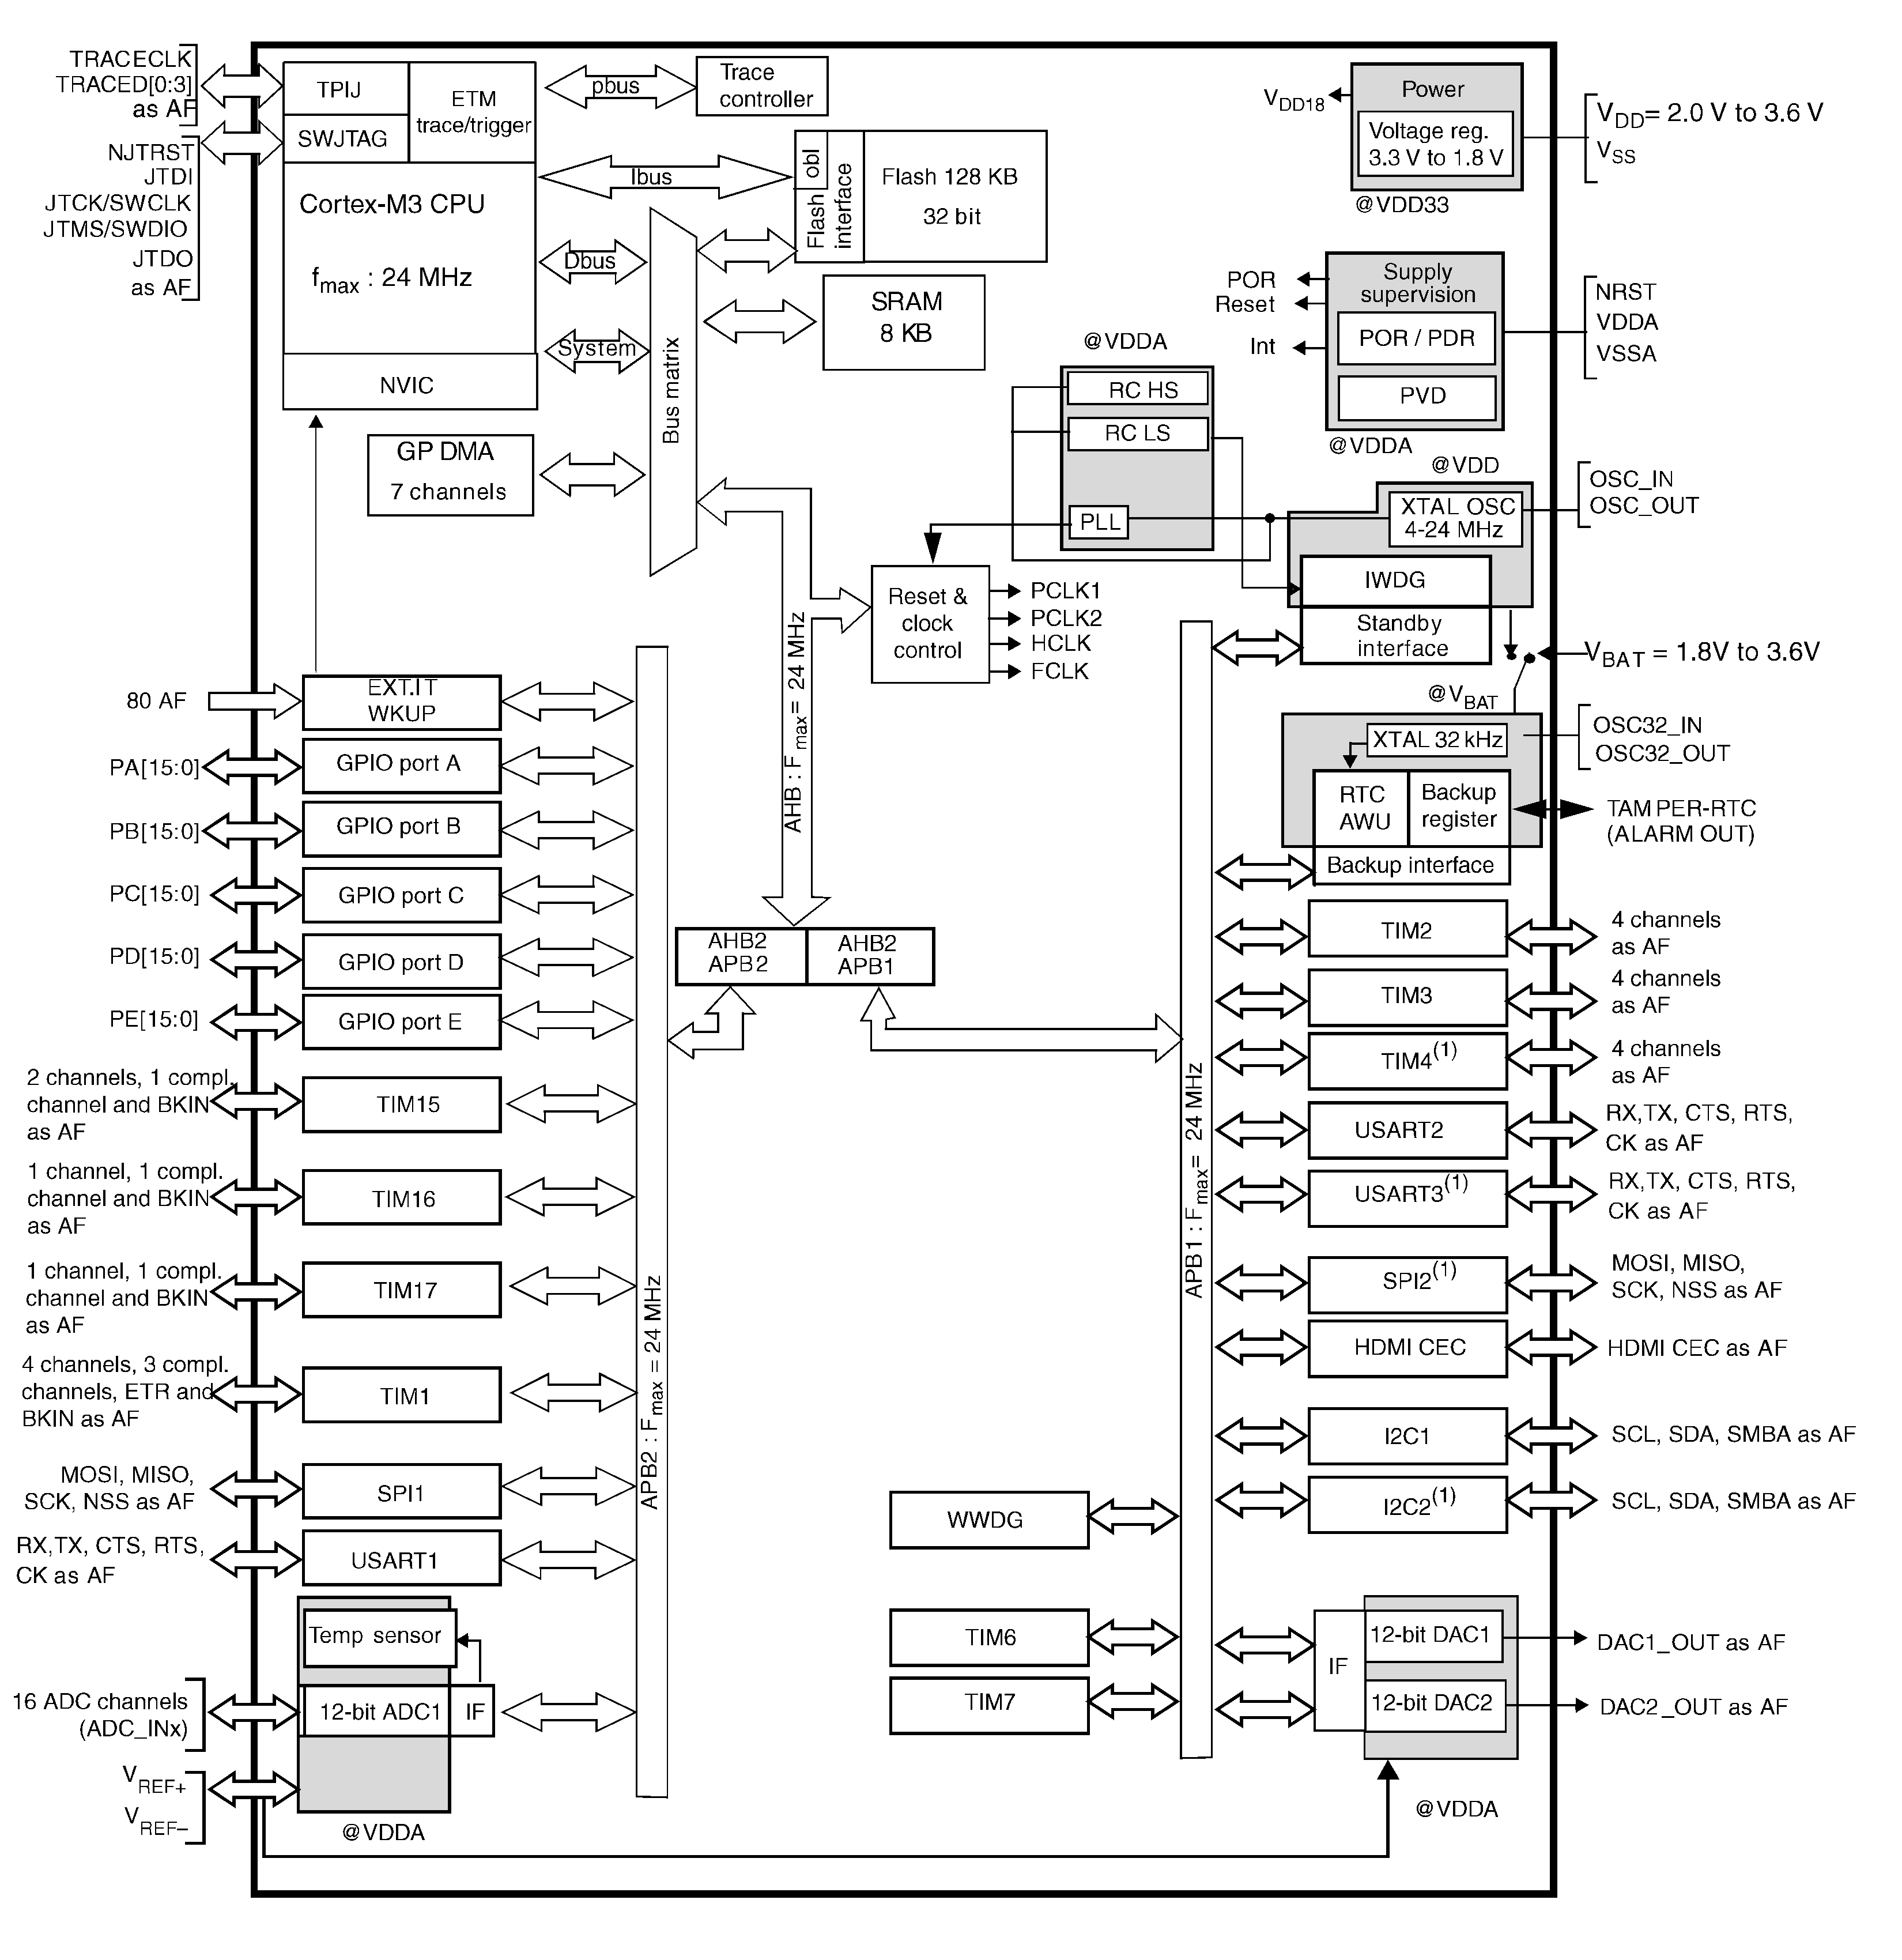
\includegraphics[width=0.65\linewidth]{img/stm32f100rbt6b}}
            \caption{Структурная схема микроконтроллера STM32F100RBT6B}
            \label{fig:stm32f100rbt6b}
        \end{sidewaysfigure}       
        
        Контроллер основан на высокопроизводительном 32 битном вычислительном
        ядре Cortex-M3 фирмы ARM.

        Cortex-M3 является стандартизованным микроконтроллерным ядром, которое
        помимо ЦПУ, содержит все остальные составляющие основу микроконтроллера
        элементы (в том числе приоритетный контроллер вложенных прерываний, 24
        битный системный таймер, интегрированный в ядро отладочный интерфейс). 

        4 гигабайтное адресное пространство Cortex-M3 разделено на четко
        распределенные области кода программы, статического ОЗУ, устройств
        ввода-вывода и системных ресурсов. Cortex-M3 выполнено по Гарвардской
        архитектуре и  имеет несколько шин, позволяющие параллельно выполнять
        такие операции как загрузка опкода, его выполнение (у МК имеется
        трехступенчатый конвеер), перемещение данных между регистрами и ОЗУ.

        Центральный процессорный элемент ядра Cortex-M3 имеет 13 регистров
        общего назначения, аппаратный 32 битный одноцикловый перемножитель,
        аппаратный делитель, а так же поддерживает два режима работы: потоковый
        режим (Thread) и режим обработчика (Handler), для каждого из которых
        можно сконфигурировать свои собственные стеки. Благодаря этому,
        появляется возможность разработки более интеллектуального программного
        обеспечения и поддержки операционных систем реального времени (ОСРВ) не
        только с кооперативной, но и с вытесняющей многозадачностью.

        Контроллер векторизированных вложенных прерываний (КВВП) может
        обрабатывать до 255 векторов, включая 15 исключений генерируемых
        процессорным ядром. КВВП также позволяет установить каждому вектору
        один из 16 уровней приоритета.

        Вход в процедуру обработки прерывания длится всего 12 машинных
        циклов, а на обработку каждого следующего вложенного прерывания
        процессор использует всего 6 циклов. Это достигнуто  за счет
        автоматического сохранения контекста прерванной программы и
        переключения стеков, выполняемых специальным микрокодом внутри ЦПУ.

        В ядро Cortex-M3 также входит 24-битный автоматически перезагружаемый
        таймер, предназначенный для генерации периодических прерываний и
        используемый ядром ОСРВ.

        Микроконтроллер имеет 16-битный таймер с возможностью управления
        трехфазным мостом силовых транзисторов. Таймер обеспечивает
        программируемое мертвое время, вход аварийной блокировки,
        настраиваемую полярность ШИМ сигнала.

        Два таймера общего назначения позволяют осуществлять обработку данных
        инкрементных энкодеров. Вычисление положения вала электродвигателя
        работает полнотью автоматически, независимо от ядра микроконтроллера.

        Семиканальный контроллер прямого доступа в память играет важную роль при
        программировании интерфейсов передачи данных, помогая существенно разгрузить
        вычислительное ядро.

        Хотя напряжение питания микроконтроллера 3,3В, практически все его
        порты ввода-вывода толерантны к напряжениям до 5В.

    \subsubsection{Описание цифровых изоляторов ADUM1300}
        ADuM1300 – трех канальные цифровые изоляторы компании Analog Devices.
        Отличительные особенности:
        \begin{itemize}
            \item низкое потребление (1.0 мА на канал на скорости до 10
                Мбит/с);
            \item двунаправленная передача данных;
            \item совместим с 3.3 В и 5.0 В питанием/уровнями логических
                сигналов;
            \item высокая скорость передачи данных: от 0 до 10 Мбит/с;
            \item максимальное искажение длительности импульса 2 нс;
            \item максимальное временное рассогласование каналов 2 нс;
            \item способность выдерживать воздействие изменяющегося входного
                синфазного сигнала, имеющего скорость нарастания более 25
                кВ/мкс;
            \item Функция активизации выходов;
            \item широкий 16 выводной SOIC корпус;
        \end{itemize}


        \begin{figure}[h!]
            \center{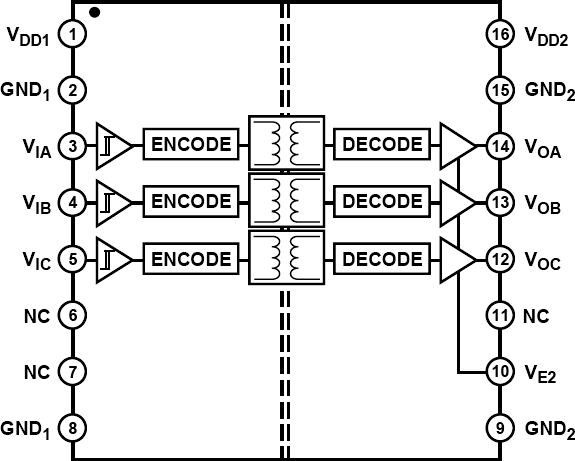
\includegraphics[width=0.8\linewidth]{img/adum1300}}
            \caption{Структурная схема цифрового изолятора ADUM1300}
            \label{fig:adum1300}
        \end{figure}

        Изоляторы семейства ADUM130X имеют три независимых канала и выпускаются
        в трех модификациях с различной пропускной способностью. Прибора
        ADuM1300 работает от однополярного источника питания, подключенного к
        любой стороне прибора, от 2,7 до 5,5 В, что позволяет обеспечить
        совместимость с низковольтными системами и произвести преобразование
        уровней сигналов через изоляционный канал. Кроме того, приборы ADUM130X
        обеспечивают низкие искажение ширины импульсов и временное
        рассогласование каналов.  Изоляторы ADUM130X имеют запатентованную
        функцию регенерации, которая гарантирует передачу статических
        параметром логических сигналов.

    \subsection{Разработка и реализация программной части системы управления АИН}
%TODO
